\documentclass{article}
\usepackage[utf8]{inputenc}
\usepackage[T1]{fontenc}
\usepackage{textcomp}
\usepackage{amsmath,amssymb}
\usepackage{lmodern}
\usepackage[a4paper]{geometry}
\usepackage{graphicx}
\usepackage{xcolor}
\usepackage{microtype}
\usepackage{hyperref}
\usepackage{diagbox}
\usepackage{booktabs}
\usepackage{listings}
\usepackage[francais]{babel}
\usepackage{algorithm}
\usepackage{algorithmic}
\definecolor{darkWhite}{rgb}{0.94,0.94,0.94}
\lstset{
  aboveskip=3mm,
  belowskip=-2mm,
  backgroundcolor=\color{darkWhite},
  basicstyle=\footnotesize,
  breakatwhitespace=false,
  breaklines=true,
  captionpos=b,
  commentstyle=\color{red},
  deletekeywords={...},
  escapeinside={\%*}{*)},
  extendedchars=true,
  framexleftmargin=16pt,
  framextopmargin=3pt,
  framexbottommargin=6pt,
  frame=tb,
  keepspaces=true,
  keywordstyle=\color{blue},
  language=C, JavaScript
  literate=
  {²}{{\textsuperscript{2}}}1
  {⁴}{{\textsuperscript{4}}}1
  {⁶}{{\textsuperscript{6}}}1
  {⁸}{{\textsuperscript{8}}}1
  {€}{{\euro{}}}1
  {é}{{\'e}}1
  {è}{{\`{e}}}1
  {ê}{{\^{e}}}1
  {ë}{{\¨{e}}}1
  {É}{{\'{E}}}1
  {Ê}{{\^{E}}}1
  {û}{{\^{u}}}1
  {ù}{{\`{u}}}1
  {â}{{\^{a}}}1
  {à}{{\`{a}}}1
  {á}{{\'{a}}}1
  {ã}{{\~{a}}}1
  {Á}{{\'{A}}}1
  {Â}{{\^{A}}}1
  {Ã}{{\~{A}}}1
  {ç}{{\c{c}}}1
  {Ç}{{\c{C}}}1
  {õ}{{\~{o}}}1
  {ó}{{\'{o}}}1
  {ô}{{\^{o}}}1
  {Õ}{{\~{O}}}1
  {Ó}{{\'{O}}}1
  {Ô}{{\^{O}}}1
  {î}{{\^{i}}}1
  {Î}{{\^{I}}}1
  {í}{{\'{i}}}1
  {Í}{{\~{Í}}}1,
  morekeywords={*,...},
  numbers=left,
  numbersep=10pt,
  numberstyle=\tiny\color{black},
  rulecolor=\color{black},Usine logicielle javascript
  showspaces=false,
  showstringspaces=false,
  showtabs=false,
  stepnumber=1,
  stringstyle=\color{gray},
  tabsize=4,
  title=\lstname,
}
\hypersetup{pdfstartview=XYZ}
\title{TD3 Théorie des graphes}
\author{}
\date{}
\begin{document}
\maketitle{}
\section*{Exercice 1}
\subsection*{Graphe G}
. \\
a : (1,20) \\
b : (8,13) \\
c : (9,12) \\
d : (10,11) \\
e : (6,15) \\
f : (7,14) \\
g : (3,18) \\
h : (4,17) \\
i : (5,16) \\
j : (2,15) \\
\subsection*{Graphe H}
. \\
a : (1,12) \\
b : (2,11) \\
c : (18,19) \\
d : (17,20) \\
e : (13,16) \\
f : (5,6) \\
g : (4,7) \\
h : (8,9) \\
i : (14,15) \\
j : (3,10) 

\section*{Exercice 2}
\subsection*{(1)}
Chaque sommet v est traité exactement une fois. \\
Le traitement de chaque sommet $o(d(v)$ donc $o(n+m)$
\newpage
\subsection*{(2)}
. \\
Arc liaison (u,v): \\
u : gris \\
v : blanc \\
d[u] est initialisé à un entier \\
f[u]=$\infty$ \\
v n'a pas de date \\
\\ 
Arc arrières (u,v): \\
u: gris (début mais pas fin) \\
v: gris \\
$d[v]<d[u]$ \\ 
\\
Arc avant (u,v): \\
u: gris \\
v: noir \\
d[u]<d[v]<f[v]
\\
Arc transverse (u,v): \\
u : gris \\
v : noir \\
f[v]<d[u]  \\
\subsection*{(3)}
\section*{Exercice 3}
Pas en relation de descendance quand ils sont dans des branches différentes. Les intervalles début et fin sont donc disjoint. Deux sommets sont en relation d'ascendances(descendances) si et seulement si $I_u \supset I_v$.
\newpage
\section*{Exercice 4}
Arc sans circuit : Parcours en profondeur dont aucun arc arrière n’est généré. \\
Fortement connexe : Toutes pairs de sommets x,y on a un chemin de x à y et un chemin de y à x. \\
\\
On identifie les Puits=${v \mid d^{+}(v)=0\}$ Pas de descendent (ici d) \\
On identifie les Sources=${v \mid d^{-}(v)=0\}$ Pas de parents (ici a) \\
On relie le Puits à la source. \\
\\
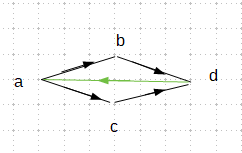
\includegraphics{Image/PS.PNG}
\\
D'une manière général on rajoutes $P \times S$ arcs. Avec P : le nombre de Puits et S : Le nombre de sources. \\
Problème : La solution est trop coûteuse. \\
\\
Il faut donc faire un super puits (relier avec les autres puits) et une super source (relier avec les autres sources). \\
Le nombre d'arc est donc : \\
$(\mid P \mid-1)+(\mid S \mid -1)+1=\mid P \mid + \mid S \mid -1$
\\
\\
Montrons maintenant que le graphe est fortement connexe. \\
Il existe un chemin de a vers b, \\
- Il existe dans G un chemin de a vers p'(un puits) \\
- Dans G' on ajoute un chemin de p vers p' (super puits) \\
- On peut le relier à s (super source) \\
- Il existe un chemin dans G qui va de s' (une source) à b \\
- Il existe un chemin de s' à s. \\ 
\\
a -> p' -> p -> s -> s' -> b \\
Faire de même pour aller de b vers a.
\section*{Exercice 5}
. \\
- Réflexive : $xRx$ $x\leq x$ \\ 
- Antisymétrique : $x \leq y$ et $y \leq x$ $\Rightarrow x=y$\\
- Transitive : $x \leq y$ et $y \leq z$ $\Rightarrow x \leq z$ \\ 
\newpage

\end{document}
